%=========================================================================
%===============================================================================

\chapter{Úvod}
Odpovídání na otázky je dobře prozkoumaný a populární úkol z oblasti zpracování přirozeného jazyka. Využití kolem nás, v běžném životě, můžeme vidět třeba u vyhledávacích nástrojů, komunikačních agentů nebo hlasových asistentů.\par 
Výzkum se v dané oblasti soustředí na metody strojového učení pro vyznačení odpovědi na otázku v daném textu. Pro trénink neuronové sítě, která by byla schopná spolehlivě vykonávat takový úkol, je zapotřebí velké množství anotovaných dat.\par 
Kromě porozumění textu jsou v oblasti důležité také algoritmy pro zhodnocení relevantnosti dokumentů používané všemi vyhledávacími nástroji a metody zpracování textu, které jsou užitečné pro optimální funkci vyhledávacích algoritmů.\par
Pro češtinu je množství i velikost dostupných datových sad oproti angličtině malé a~je tedy obtížné dosáhnout s ní podobných výsledků, jako u jazyků s mnoha zdroji (angličtina, němčina, francouzština \dots). Obzvlášť v kontextu toho, že pro většinu úkolů na poli zpracování přirozeného jazyka se v posledních letech nejlépe osvědčily velké modely předtrénované na velmi rozsáhlých korpusech textu. Ty pro češtinu prozatím bohužel nejsou dostupné v~dostatečné kvalitě.\par
V této práci se snažím otestovat přístup, který využívá strojový překlad češtiny do angličtiny, aby mohlo být použito jednoho z robustních předtrénovaných modelů pro porozumění textu. Kromě metod pro porozumění textu a extrakci odpovědi v práci rozebírám algoritmy řazení dokumentů dle jejich relevance k otázce. Jako báze znalostí pro systém schopný na otázky odpovídat je použita česká Wikipedie, jejíž články jsou pro nalezení vhodné odpovědi prohledávány.\par
Začal jsem popsáním metod pro zpracování textu v kapitole \ref{text_processing}. Popsány jsou zde metody reprezentace slov a způsoby zpracování textu vhodné pro porozumění textu a pro algoritmy řazení relevantních dokumentů.\par
Kapitola \ref{language_comprehension} se zabývá popisem neuronových sítí pro porozumění textu a extrakci odpovědi. Popsány jsou zde moderní architektury a modely použité v práci. V kapitole \ref{available_datasets} jsou poté popsány datové sady vhodné pro trénink a vyhodnocení výsledného systému.
Následuje kapitola \ref{design_and_implementation}, kde je popsán návrh a implementace systému založeného na zmíněných postupech a kapitola \ref{system_evaluation}, kde je výsledný systém vyhodnocen s použitím standardních metrik.




%=========================================================================
%===============================================================================

\chapter{Reprezentace slov a zpracování textu}
\label{text_processing}

Předtím, než se vrhneme na vysvětlení poměrně složitých jazykových modelů a vyhledávacích algoritmů, bude v této kapitole vysvětleno pár základních pojmů a technik.\par 
Počítač lidské řeči na elementární úrovni příliš nerozumí, jsou mu ale mnohem bližší čísla a statistika. Proto musíme nejdříve porozumět tomu, s jakou reprezentací slov moderní jazykové modely pracují a do jaké podoby je tedy potřeba zdrojový text dostat. Vysvětleny jsou tedy termíny související s reprezentací slov pomocí vektorů, neboli \uv{word embeddings} a tokenizace textu.\par 
Také je potřeba prozkoumat možnosti zpracování textů a slov na jejich morfologické úrovni. Tato úloha je na pomezí informatiky a lingvistiky a používají se pro ni speciální nástroje. Použité techniky jako lemmatizace a odstranění stop-slov zajistí optimální funkčnost některých použitých algoritmů.\par
Po přečtení kapitoly by měl být čtenář teoreticky vybaven pro pochopení konceptů vysvětlených v kapitolách \ref{language_comprehension} a \ref{document_indexing}, které na zde popsaných technologiích staví a částečně se s nimi překrývají.

%=========================================================================
\section{Reprezentace slov}
\label{reprezentace_slov}
Jak už bylo řečeno, je složité pracovat s textem v takové podobě, na jakou jsou lidé zvyklí. Počítač v ní nedokáže vidět důležité sémantické souvislosti, které jsou pro přirozený jazyk tak důležité. Musíme tedy z textu a slov v něm získat nějakou matematickou reprezentaci, která je počítači bližší a se kterou dokáží dále pracovat neuronové sítě. \par
Pro takovou reprezentaci jsou nejpoužívanější vektory pevně dané dimenze známé jako \uv{word embeddings}. Pro představu například (běžně) 300 desetinných čísel pro popis každého slova v textu. Vektory slov ve slovníku nesou důležitou informaci o sémantické příbuznosti jednotlivých slov. Po promítnutí do spojitého prostoru jsou si vektory, které reprezentující sémanticky podobná slova, blízko, jak zobrazuje obrázek \ref{word_embeddings}.\par
Po aplikaci těchto myšlenek zmíněných v článcích \cite{mikolov2013embeddings} a \cite{mikolov2013_2} byl zaznamenán výrazný pokrok v úlohách z oblasti zpracování přirozeného jazyka, jako strojový překlad, porozumění textu, odhad emocí, klasifikace atp.
Vektory reprezentující slova jsou většinou získávány analýzou rozsáhlých textových korpusů. Snaží se zachytit sémantickou blízkost slov na základě jejich koexistence v podobných kontextech.\par 
Například slova \emph{pohovka} a \emph{gauč} se nejspíše budou vyskytovat v podobných situacích, protože jsou to synonyma a jejich sémantika je téměř totožná.\par
Výsledné vektory nám poté umožňují provádět se slovy také velmi zajímavé matematické operace, jako je sčítat, nebo odčítat a je schopen zachytit velmi zajímavé vztahy jako například:
\begin{center}
[Král] $-$ [Muž] $+$ [Žena] $=$ [Královna]\\
\medskip
nebo\\
\medskip
[Paříž] $-$ [Francie] $+$ [Čína] $=$ [Peking]
\end{center}

V následující části budou popsány vlastnosti a nejznámějších metod pro získání vektorových reprezentací.

\begin{figure}[hbt]
	\centering
	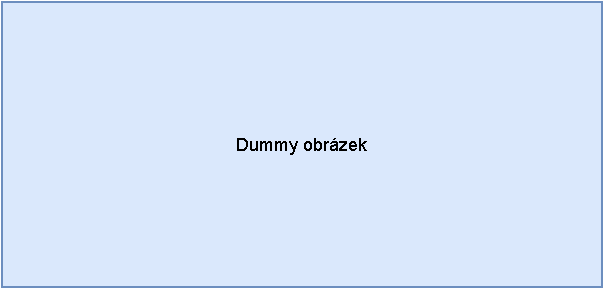
\includegraphics[width=4.0in, height=1.7in]{obrazky/dummy_pic.pdf}
	\caption{Dummy picture - znazorneni vektoroveho prostoru}
	\label{word_embeddings}
\end{figure}
%=========================================================================

\subsection{Word2vec}

Word2vec je technika prezentována v článku \cite{mikolov2013embeddings} schopná naučit se vektorové reprezentace pomocí prediktivního modelu neuronové sítě. Základním konceptem dvou přístupů, které se pro trénink modelu používají, je predikce slov na základě sousedních slov v tzv. kontextovém okně, které se postupně posouvá. Dostáváme tedy pro každé slovo pravděpodobnost, se kterou se bude vyskytovat v blízkosti slova cílového.\par
První model používaný pro trénink word2vec vektorů se nazývá Continuous Bag of Words, neboli CBOW. Neuronová síť se trénuje hádáním chybějícího slova v kontextu známých sousedním slov kontextového okna.\par
Druhá metoda funguje funguje na opačném principu a nazývá se Continuous Skip-gram Model. Na základě současného slova se tedy model snaží předpovědět slova v určitém vzdálenosti před, i po současném slově, v závislosti na velikosti kontextového okna. Tato metoda se z článku \cite{mikolov2013embeddings} jeví jako o něco úspěšnější a je dále zdokonalena v článku \cite{mikolov2013_2}.\par
Na obrázku \ref{cbow_and_skipgram} můžeme vidět rozdíl v tom, jak projekční vrstva transformuje vstup na výstup v případě obou architektur.

\begin{figure}[hbt]
	\centering
	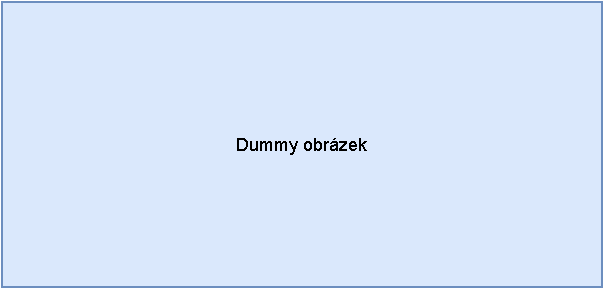
\includegraphics[width=0.45\linewidth, height=2in]{obrazky/dummy_pic.pdf}\hfill
	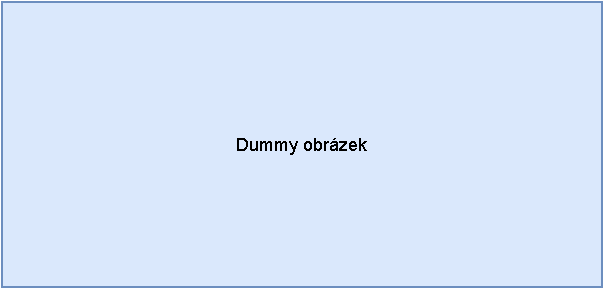
\includegraphics[width=0.45\linewidth, height=2in]{obrazky/dummy_pic.pdf}
	\caption{Obrázek cbow a skipgram}
	\label{cbow_and_skipgram}
\end{figure}

%=========================================================================

\subsection{GloVe}

GloVe, neboli Global Vectors for Word Representation je technika prezentována v článku \cite{GloVe}. Výsledkem je vektorový prostor o pevně dané dimenzi stejně, jako u word2vec reprezentace. Liší se však způsobem získání daných reprezentací.\par Zatímco word2vec je prediktivní model, GloVe je spíše modelem statistickým. Klade tedy důraz hlavně na počet výskytů slov a počet jejich výskytů v podobných kontextech. Dostaneme tedy nějakou matici společných výskytů slov v korpusu.\par
Jeho hlavní výhodou je, že se nesoustředí pouze na slova v těsném kontextu, jak už slovo \emph{Global}, ukryté v GloVe, napovídá. Reprezentace je tedy schopná zachytit sémentické souvislosti v širším kontextu, ale základní idea není konceptu word2vec příliš daleko.

%=========================================================================

\subsection{Wordpiece embeddings}
\label{wordpiece_embb}
Wordpiece je prediktivní technika prezentována článkem \cite{wordpiece} v roce 2016 (původně představeno pro strojový překlad) a používána modely popsanými v sekci \ref{bert_albert}.\par
Hlavním záměrem přístupu je lépe se vypořádat s ojedinělými slovy tak, že jsou slova rozdělena do již známých \emph{podslov}. Nabízí tím kompromis mezi \emph{word embeddings} pro celá slova a tzv. \emph{character embeddings} pro jednotlivé znaky.\par
Slovník je nejprve naplněn všemi znaky v textu a jazykový model je na tomto slovníku trénován. Z výsledného slovníku modelu je poté sestaven slovník nových kombinací jednotlivých znaků tak, aby se zlepšila úspěšnost na trénovací datové sadě. Postup se opakuje, dokud nenarazíme na limit minimální velikosti slovníku, nebo je rozdíl mezi úspěšností jednotlivých iterací modelu příliš malý.

%=========================================================================
\section{Tokenizace a předzpracování}
\label{preprocessing}
Zpracování textu je důležitou součástí oblasti zpracování přirozeného jazyka. S textem se totiž pracuje lépe, pokud jsme schopni odstranit některé záludnosti a nadbytečnosti přirozeného jazyka a dostat ho do podoby, který je pro automatické zpracování vhodnější. Jednotlivé nástroje pro efektivní zpracování textu v práci jsou poté uvedeny v části \ref{pouzite_nastroje}.\par
První část této sekce navazuje na část \ref{reprezentace_slov} o reprezentaci jednotlivých slov textu a zabývá se postupem rozdělení textu na tzv. \emph{tokeny}, které mohou být později převedeny na jejich vektorovou reprezentaci.\par
Druhá část je věnována postupům pro zpracování a pokud možno normalizaci textu pro optimální využití vyhledávacích algoritmů. Statistické metody využívány těmito algoritmy jsou efektivnější, pokud jsou z textu odstraněny například slova nesoucí zanedbatelnou informaci. Mohou být také zmateny různými tvary daných slov.

\subsection{Tokenizace vstupního textu}
\textbf{Tokenizace} je převod textu jako posloupnosti jednotlivých znaků na posloupnost jednotlivých tokenů. Například rozdělení textu \uv{Adam šel po škole domů.} na posloupnost jednotlivých tokenů:
\begin{center}
    \_Adam $+$ \_šel $+$ \_po $+$ \_škole $+$ \_domů $+$ \_.
\end{center}
Primitivní přístup je rozdělení textu pomocí bílých znaků a interpunkčních znamének, který ale nebere ohled např na tečky uprostřed zkratek v angličtině a těžko se vypořádává se složeninami. Získané tokeny je pak taky třeba normalizovat pro následný převod na word embeddings.\par
V přístupu uvedeném v sekci \ref{wordpiece_embb} jsou slova děleny na tokekeny podle toho, která podslova v daném textu jsou slovníku známy. Můžeme si uvést příklad z angličtiny, s jímž podobným se ještě jistě setkáme i v sekci \ref{bert_albert}. Věta \uv{I like playing.} by tedy byla převedena na následující tokeny:
\begin{center}
    \_I $+$ \_like $+$ \_play $+$ \_ing $+$ \_.
\end{center}
Na uvedeném případě je vidět hlavně převedení posloupnosti znaků \uv{playing} na dvě podslova (tokeny) \emph{play} a \emph{ing}.

\subsection{Normalizace délky textu a rozdělení do vět}
V kontextu práce je normalizací délky textu myšlena jakási standardní maximální délka dokumentu, který je později předložen readeru k vyznačení správné odpovědi. Tento přístup je užitečný ze několika důvodů.\par
Algoritmy pro řazení dokumentů dle relevance sice berou na relativní délku každého textu ohled, nicméně některé články jako \cite{bm25_too_long} nasvědčují, že můžou být příliš dlouhé dokumenty znevýhodněny. Článek \cite{bm25_too_long} sice představuje úpravu klasického algoritmu pro minimalizaci tohoto problému, v práci jsou ale i další důvody, proč je vhodné délku jednotlivých odstavců normalizovat.\par
Model pro vyznačení správné odpovědi v textu je trénován na datové sadě, která příliš dlouhé dokumenty nebere v úvahu\footnote{Pro každou otázku je jen jeden odstavec kontextu, ne celý článek z Wikipedie.} a jak je naznačeno v článku \cite{QA_long_multiple_span}, není na dlouhých dokumentech příliš úspěšný.\par
Dalším důvodem je snaha nepřekládat pro účel vyznačení správné odpovědi příliš dlouhé důvody textu.\footnote{Hlavně kvůli určitým omezením dostupných nástrojů pro překlad.}

\paragraph{Proč rozdělit text do vět?}
Předpokládejme, že je text již rozdělen do jednotlivých odstavců. Pro každý odstavec je kontrolována jeho délka, jestli nepřesahuje délku maximální. Pokud bude maximální délka odstavce překročena, může být sice rozdělen jednoduše na poloviny, na třetiny a tak dále podle potřeby, bude tím ale ztracena velká část kontextu při rozdělení některých vět v půlce.\par
Pro takový případ je vhodné vědět, kde jednotlivé věty začínají a končí, aby bylo možné jednotlivé odstavce případně smysluplně rozdělit. Vhodné je také zařídit, aby se jednotlivé rozdělené \uv{pododstavce} částečně překrývaly a obsahovaly třeba 3 poslední věty odstavce předchozího, pro maximální zachování původního kontextu.

\subsection{Převod na malá písmena}
\label{prevod_na_mala}
Převod na malá písmena je sice velmi jednoduchý, ale přesto užitečný úkol. Při psaní otázky na klávesnici je velmi pravděpodobně, že pomyslný uživatel napíše \uv{sssr} místo \uv{SSSR} nebo \uv{Albert} místo \uv{ALBERT}, ale bylo by vhodné, aby byly nalezeny dokumenty obsahující obě varianty. Stejně tak může dojít k nestandardnímu užití malých/velkých písmen v některém z dokumentů.\par
Pro některé případy může převod na malá písmeny znamenat ztrátu části kontextu. Například \emph{Malá Strana} X \emph{malá strana}, kde velké písmeno indikuje vlastní jméno (městskou část). Vhodné je to tedy pouze v některých případech.

\subsection{Odstranění stop slov}
\label{stopwords}
Ve zpracování přirozeného jazyka jsou \emph{stop slova} většinou souborem nejčastěji používaných slov v daném jazyce \cite{wiki:stopwords}. Většinou jsou odstraňována, protože kvůli jejich vysokému výskytu nesou menší informační hodnotu a jejich odstranění vede k lepší funkci vyhledávacích algoritmů \cite{bm25_improvements}.\par
Nejužívanější slova daného jazyka je možno například ve frekvenčních seznamech jako \cite{wiki:frekvencni_seznam}, který obsahuje 100 nejpoužívanějších slov v češtině. Získaný seznam je vhodné kriticky zhodnotit a vyčlenit z něj některá slova, která by pro vyhledávání mohla mít kritický význam.\footnote{Příklad: \uv{první}, \uv{země}, \uv{člověk} \dots} Většinou je zanedbatelná alespoň většina spojek, předložek či zájmen. Typickými příklady stop slov pro češtinu jsou: být, a, se, v, že \dots

\subsection{Získání lemmat}
\textbf{Lemmatizace} je druh zpracování textu, při kterém je pro každé slovo nalezen základní tvar, tzv. \emph{lemma}.\footnote{Podobným postupem je \emph{stematizace}, která ale algoritmicky pouze odstraní koncovky a předpony pro nalezení slovního kmene. Lemmatizátor pro nalezení základních tvarů používá morfologický slovník.}
\begin{center}
    ulicí běžely děti $\longrightarrow$ ulice běžet dítě\\
    ostrovy Středozemního moře $\longrightarrow$ ostrov Středozemní moře
\end{center}
Pro získání lemmat se používají speciální nástroje pro zpracování přirozeného jazyka. \emph{Lemma\-tizátory} mohou poskytovat také některé doplňkové informace o mluvnichkých kategoriích jako rod, pád nebo slovní druh. Hlavním úskalím lemmatizátorů je mnohoznačnost jazyků jako je čeština, kdy může být více základních tvarů daného slova dle kontextu \cite{wiki:lemmatizator}.\par
Využití lemmatizace je různé, ale v případě této práce je podobné, jako účel postupu uvedeného v sekci \ref{prevod_na_mala}. Jednoduše se hodí, když pro dotaz obsahující \uv{\dots Liparských ostrovů} budou nalezeny i dokumenty obsahující základní tvar hledaného výrazu \uv{Liparské ostrovy}\par
Lemmatizace je také užitečným nástrojem při odstranění stop slov, kdy můžeme například odstranit všechny tvary slovesa \uv{být}, zatímco seznam stop slov může obsahovat pouze jeho základní tvar.


%=========================================================================
%===============================================================================

\chapter{Strojové učení pro extrakci odpovědi}
\label{language_comprehension}

Rozmach strojového učení umožnil obrovský pokrok v oblastech NLP jako strojový překlad, rozpoznání entit, generování textu nebo také odpovídání na otázky. Proto na tomto přístupu staví všechny nejmodernější metody a tímto směrem se také ubírá výzkum.\par
Účelem této kapitoly je vysvětlit čtenáři, jak fungují neuronové sítě a jakým způsobem dokáže počítač porozumět textu a naučit se vyznačit v textu odpověď na danou otázku.\par
Nejprve budou ve zkratce vysvětleny principy fungování a učení neuronových sítí. Poté budou rozebrány nejznámější architektury neuronových sítí používané pro vypořádání se s úkoly na poli zpracování přirozeného jazyka a nakonec budou popsány nejmodernější modely, které na nich staví.
\bigskip

%=========================================================================
\section{Neuronové sítě}
\label{neuronove_site}
V této části bude vysvětlen princip fungování neuronových sítí. Informace v sekci byly převzaty z článku \cite{neural_nets} a z prezentací Stanfordského kurzu NLP.\footnote{Dostupné z: \url{http://web.stanford.edu/class/cs224n/}}\par
Neuronové sítě si můžeme zjednodušeně představit jako velkou funkci s obrovským množstvím parametrů, která přetváří vstupy na výstupy. V průběhu tréninku neuronové sítě se postupně všechny parametry optimalizují tak, aby síť přetvářela vstupy na výstupy co nejlépe.\par
Fungují tu tři základní jednoduché vrstvy(\ref{three_layers}). Vstupní, skrytá (zde probíhá proces přetváření vstupů) a výstupní, na které se přetvořený vstup objeví. Skrytá vrstva se navíc běžně skládá z mnoha dalších vrstev.\par
Každá z těchto vrstev, ať už je vstupní, výstupní, nebo skrytá, se skládá z dalších primitiv a ty jsou nazývány jak jinak, než neurony. Každý neuron v každé vrstvě je propojen s každým neuronem vrstvy další, a tak je propojena celá síť.

\begin{figure}[hbt]
	\centering
	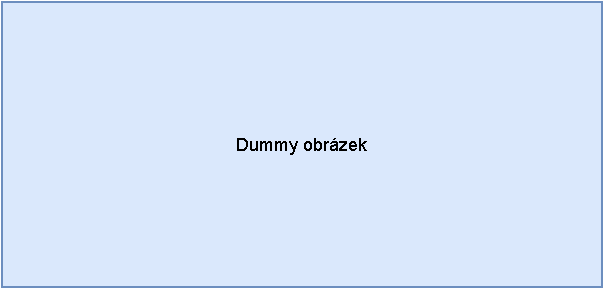
\includegraphics[width=4.0in, height=2in]{obrazky/dummy_pic.pdf}
	\caption{Dummy picture - znázornění neuronové sítě se třemi vrstvami a váhami.}
	\label{three_layers}
\end{figure}

\subsection{Umělý neuron a aktivační funkce}
Umělý neuron je primitivní jednotka inspirována neuronem skutečným. Ten vypadá asi tak, že má tělo, do kterého přichází krátkými výběžky, tzv. \emph{dendrity} elektrické signály z ostatním neuronů. Z těla tohoto neuronu pak vychází jediný dlouhý výběžek, tzv. \emph{axon}. Neuron se tedy na základě signálů, které do něj přichází dendrity rozhodne (na základě nějaké minimální hranice přijatého signálu), zda-li bude, nebo nebude vysílat signál dál \cite{wiki:neuron}.\par
Funkce umělého neuronu je analogická. Jak už bylo popsáno v úvodu sekce \ref{neuronove_site}, každý neuron je propojen s každým neuronem vrstvy předcházející i vrstvy další. Na rozdíl od skutečného neuronu má tedy \uv{více axonů}, kterými je propojen s další vrstvou.\par
Každé propojení mezi každým neuronem má svoji váhu \emph{w}, která ovlivňuje důležitost jednotlivého vstupu do neuronu. Každý neuron má pak svůj práh \emph{B} a aktivační funkci. Výstupem neuronu je tedy vážená suma vstupů do neuronu s přičteným prahem a aplikovanou aktivační funkcí, neboli 
$$F({\sum_{i=1}^n ({x_n}w_n)} + B)$$
kde $x_n$ je neuron předcházející vrstvy, $w_n$ je váha jeho propojení, $B$ je práh aktuálního neuronu a $F$ je aktivační funkce. Znázornění vah propojení a jednotlivých neuronů je vyznačeno na obrázku \ref{three_layers}.\par
Všechny propojení jednotlivých neuronů a jejich prahy v dávají dohromady parametry neuronové sítě, které jsou v průběhu tréninku optimalizovány pro každý neuron zvlášť. Pro síť, jako je na obrázku \ref{three_layers} je to třeba 30 jednotlivých vah propojení a 8 prahů jednotlivých neuronů (skryté a výstupní vrstvy), tedy 38 parametrů v tak jednoduché síti.\par
\textbf{Aktivační (přenosová) funkce} rozhoduje, jestli bude daný neuron aktivován. Skutečný neuron má, zdá se, funkci skokovou. Umělé neurony však používají funkce s postupnou aktivací. Běžné jsou tři (čtyři) základní varianty aktivačních funkcí: 

\begin{itemize}
    \item (Skoková)
    \item Sigmoidální
    \item Hyporbolické tangenty
    \item ReLU (Rectified Linear Unit)
\end{itemize}

Funkce jsou znázorněny na obrázku \ref{aktivacni_funkce}. Vhodnost použití každé z nich může být různé. Výhodou sigmoidální funkce je normalizace výstupu do rozmezí $(0,1)$. Nejpoužívanější funkcí pro skrytou vrstvou je však funkce ReLU. Kvůli její charakteristice je aktivováno méně neuronů, což vede k rychlejšímu tréninku a konvergenci. Použití ReLU funkce je také méně výpočetně náročné \cite{medium:activation_function}.


\begin{figure}[hbt]
	\centering
	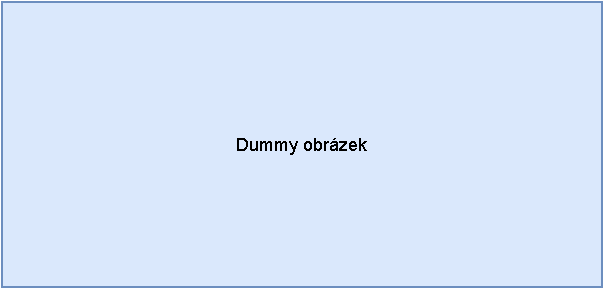
\includegraphics[width=0.33\linewidth, height=1.5in]{obrazky/dummy_pic.pdf}\hfill
	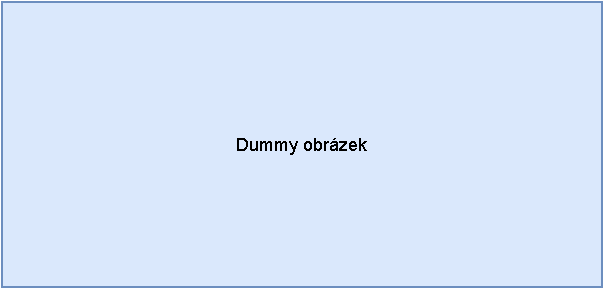
\includegraphics[width=0.33\linewidth, height=1.5in]{obrazky/dummy_pic.pdf}\hfill
	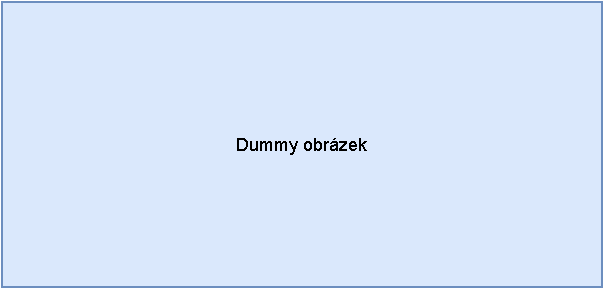
\includegraphics[width=0.33\linewidth, height=1.5in]{obrazky/dummy_pic.pdf}\hfill
	\caption{Obrázek sigmoid, tanh a relu funkce}
	\label{aktivacni_funkce}
\end{figure}


\subsection{Dopředná a zpětná propagace}
Proces, kdy se opakovaně ze vstupů počítá výstup každého neuronu v dané vrstvě a stejně tak pro každou následující vrstvu, se nazývá dopředná propagace. Tímto postupem se postupně hodnoty vstupní vrstvy přetvoří na hodnoty ve vrstvě výstupní a může se určit, jak byla síť úspěšná.\par
Pro určení úspěšnosti každé takové iterace neuronové sítě se používá nákladová funkce (anglicky cost function pro jednu iteraci, loss function pro průměr všech), která udává jediné číslo charakterizující úspěšnost modelu. Nejznámější nákladovou funkcí je Střední kvadratická chyba (anglicky Mean Squared Error - MSE). Cílem je hodnotu této nákladové funkce postupně minimalizovat.\par \medskip
Postup optimalizace jednotlivých parametrů neuronové sítě pro zajištění minimalizace nákladové funkce se nazývá \textbf{zpětná propagace}. Je to v podstatě opačný průchod neuronovou sítí, který má za úkol zjistit, které neurony se největší mírou podílely na výsledné chybě. Snížením významu těchto neuronů můžeme dosáhnout lepší úspěšnosti celé sítě. Naopak můžeme zvýšit význam propojení s neurony, které výstup ovlivnily pozitivně.\par
Základem tohoto výpočtu je, že chyba každého výstupního neuronu je vstupem parciální derivace vzhledem ke každému z jeho vstupů. Celý postup zpětné propagace je velmi složitý a pro intuitivní pochopení problematiky není klíčový, proto tu nebude podrobně rozebrán.\par
Celý postup zpětné propagace je opakován a parametry neuronové sítě jsou postupně optimalizovány.\par \medskip
Trénink neuronové sítě tedy probíhá následovně. Síti s náhodně inicializovanými parametry je předložena část dat z trénovací datové sady. Ty jsou pomocí dopředné propagace prostupem přes skrytou vrstvu přetvořeny na výstupy a tím získány predikce neuronové sítě. Predikce jsou porovnány se základní pravdou (tzv. \emph{ground truth}) a nákladovou funkcí je vyjádřeno, jak byly predikce daleko od pravdy. Pomocí zpětné propagace jsou postupně upraveny všechny parametry neuronové sítě.\par
Postup je opakován, dokud úbytek nákladové funkce mezi jednotlivými iteracemi nezačne dlouhodobě stagnovat, nebo dokud nedosáhneme požadovaného počtu epoch.\par
Při nesprávném tréninku neuronové sítě může dojít k podtrénování (underfitting), nebo přetrénování (overfitting). Problémy při tréninku souvisí s tzv. hyperparametry, mezi které patři počet skrytých vrstev, velikost modelu nebo \emph{learning rate}\footnote{Konstanta určující velikost kroku při každé iteraci zpětné propagace při úpravě parametrů neuronové sítě.}. Pomoct může také množství trénovacích dat nebo počet trénovacích epoch.

%=========================================================================
\section{Nejlepší architektury pro porozumění textu}
V této sekci budou popsány dvě nejznámější a nejpoužívanější architektury používané pro zpracování přirozeného jazyka. Rozšiřují koncepty prezentované v sekci \ref{neuronove_site} a snaží se překonat problémy, které tradiční model představuje.\par
První model v části \ref{lstm} využívá k překonání ztráty kontextu rekurentní neuronové sítě. Druhý model v části \ref{transformers} spoléhá na paralelní zpracování a vzájemnou pozornost mezi otázkou a kontextem.

\subsection{Long short-term memory}
\label{lstm}
Informace v této sekci byly převzaty z originální práce \cite{LSTM}, která architekturu představuje a ze článku \cite{understandingLSTM}.\par
LSTM, neboli Long Short-term Memory je speciální druh \emph{rekurentní} neuronové sítě, který se částečně vypořádává s problémem ztráty kontextu v delším úseku textu. Jednoduše řečeno, při učení neuronové sítě bychom byli rádi, aby pochopení současné věty dokázala ovlivnit i věta předcházející.\par

\begin{figure}[hbt]
	\centering
	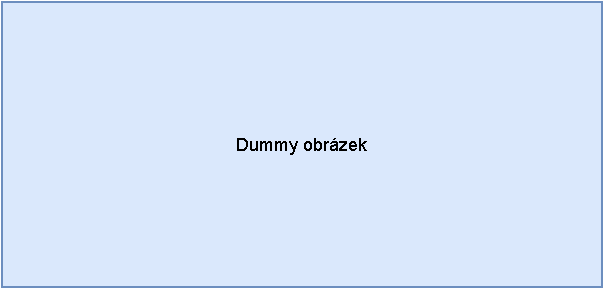
\includegraphics[width=4.0in, height=1.1in]{obrazky/dummy_pic.pdf}
	\caption{dummy obrázek - schéma RNN}
	\label{RNN}
\end{figure}

Nejprve bude vysvětlen princip \textbf{rekurentní neuronové sítě} (dále RNN - Recurrent Neural Network).
Jejich hlavním úkolem je vypořádat se se zpracováním sekvenčních dat, jako je text. Oproti například rozpoznávání vzorů v obrázcích není možné pohlížet na každé slovo v textu zvlášť. Slovo/slova předcházející by měly ovlivnit slovo současné. Stejně tak by měly následující slova ovlivnit význam slova současného (obousměrné rekurentní sítě).\par
Schéma jednoduché RNN je vidět na obrázku \ref{RNN}. Zjednodušeně je to tedy více jednoduchých neuronových sítí propojených za sebe. Vstupem každé sítě $h_n$ je výstup předchozí sítě $h_{n-1}$ a slovo $x_n$. Výstup $y_n$ je potom vstupem do další jednotky $h_{n+1}$.\par
Analogicky funguje obousměrná RNN, které je propojená i v opačném směru. Vstup je zpracováván od konce a pro současné slovo je tedy brán v úvahu i kontext slova nadcházejícího, jak je vidět na obrázku \ref{bidirRNN}.\par

\begin{figure}[hbt]
	\centering
	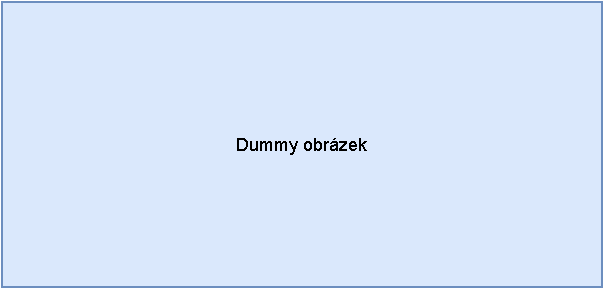
\includegraphics[width=4.0in, height=1.5in]{obrazky/dummy_pic.pdf}
	\caption{dummy obrázek - schéma obousměrné RNN}
	\label{bidirRNN}
\end{figure}

\textbf{LSTM} (Long Short-term Memory) představuje vylepšení standardní RNN.\par \smallskip
Mějme model, který má za úkol předpovědět následující slovo ve větě. Pokud se kontext potřebný pro predikci nachází v těsné blízkosti předpovídaného slova (př.: \uv{vychlazené mléko z \emph{lednice}}), je i běžná RNN schopná si souvislost propojit. Pro příklad, kdy je kontext \uv{dále v minulosti} (př.:\uv{Učím se od 6 let anglicky \dots Vzhledem k těmto okolnostem plynule ovládám \emph{angličtinu}}) není RNN schopná naučit se tuhle souvislost mezi kontextem a hledaným slovem.\par \smallskip
LSTM je tedy narozdíl od klasické RNN navržená tak, aby byla schopná pamatovat si dlouhodobé souvislosti v textu při sekvenčním zpracování. Řeší tím tzv. \emph{problém mizejícího gradientu}.\par
Model má stejnou opakující se strukturu jako RNN, rozdíl je však v komplexnosti opakující se jednotky (či buňky). Struktura naznačená na obrázku \ref{lstm_cell} je poměrně složitá a jejím hlavním komponentem jsou tzv. \emph{brány}. 

\begin{figure}[hbt]
	\centering
	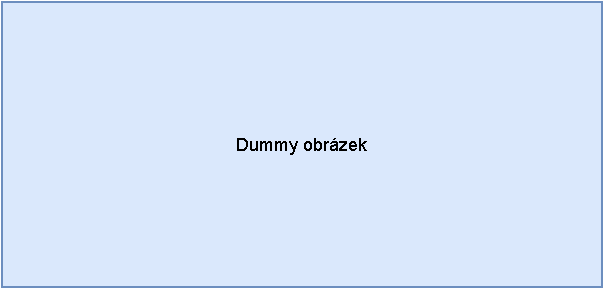
\includegraphics[width=3.0in, height=1.5in]{obrazky/dummy_pic.pdf}
	\caption{dummy obrázek - schéma lstm buňky}
	\label{lstm_cell}
\end{figure}

Brány jsou v LSTM buňce celkem tři. Každá je složena z vrstvy neuronové sítě se sigmoidální funkcí a násobícího operátoru. Brána je komponentem určujícím, kolik informace je možno propustit. Brány budou popsány zleva doprava.\par
První, tzv. zapomínací brána určuje, kolik vstupní informace je zahozeno\footnote{Výstupem je číslo v rozmezí (0,1), kde 0 znamená \uv{všechno zahodit} a 1 znamená \uv{všechno propustit}.}. Druhá, tzv. vstupní brána, určí, které hodnoty skrytého stavu buňky budou aktualizovány a vrstva s funkcí \emph{tanh} rozhodne o nových kandidátních hodnotách, které po kombinaci s výstupem sigmoidální vrstvy vytvoří nový skrytý stav buňky. Poslední bránou je výstupní, která spojuje informaci z brány zapomínací a vnitřním stavem buňky a vytváří tím tedy výstup dané buňky.\par
Jednotlivé LSTM buňky jsou za sebou sekvenčně propojeny stejně jako RNN. Při použití dvou LSTM sítí s tou druhou propojenou v opačném směru získáme obousměrnou LSTM síť. Výstupy obou sítí jsou poté pro získání výstupu zřetězeny.

\subsection{Transformers}
\label{transformers}
Informace v této sekci byly převzaty z originální práce \emph{Attention Is All You Need} \cite{Transformers}, práce \cite{attention_mechanism} a článku \cite{Transformers-explained}. Sekce popisuje Transformer model používaný pro zpracování přirozeného jazyka a mechanismus pozornosti, který s ním úzce souvisí.\par
Přístup použitý tímto modelem se dokázal oprostit od rekurentních modelů jako LSTM a nahradil je na poli zpracování přirozeného jazyka jako nová state of the art architektura. Transformers nepoužívá sekvenční zpracování slov, ale zpracování paralelní.\par
Jeho nejdůležitější myšlenkou je tzv. \textbf{mechanismus pozornosti} (anglicky \emph{attention mechanism}) představený článkem \cite{attention_mechanism} původně pro strojový překlad. Mechanismus pozornosti se však dále rozvíjel a popularizoval do dalších odvětví strojového učení. Stručně bude tedy popsán.\par \medskip

Mechanismus vezme vektory dvou vět přirozeného jazyka naráz a sestaví z nich \emph{key(\textbf{K})-value(\textbf{V})} a \emph{query(\textbf{Q})} matice (řádek -- vektor pro každé vstupní slovo). Ty vzniknou vynásobením vstupní word embedding matice speciální váhovou maticí, jejíž parametry se natrénují. Na matice jsou poté aplikovány následující operace pro získání výstupu attention mechanismu

\begin{equation}
    \label{attention_dot_product}
    softmax(\frac{Q \times K}{k})\times V
\end{equation}

kde k je podle \cite{Transformers} konstanta 8 (mohly by bý stanoveny i jiné hodnoty) a softmax funkce pro normalizaci výstupu do rozmezí (0,1).\par
Vektory pro všechny vstupní slova respektive vstupní matice K, V a Q mohou být ze stejné věty. Potom se používá termín \textbf{self-attention}.\par
Tím je určeno, která část vstupu je relevantní (self-attention), nebo například která část dokumentu je relevantním kontextem dané otázky.\par
Jednoznačnou výhodou mechanismu pozornosti je, že je schopen podívat se na celý kontext naráz (narozdíl od RNN, která prochází vstup sekvenčně) a vyznačit v něm důležité pasáže. Tímto se zbavuje problému mizejícího gradientu.\par\medskip

\textbf{Transformer} enkodér\footnote{Enkodér je část modelu, která vytvoří z vektorů jednotlivých slov na vstupu vektor celého vstupního textu, reprezentující jeho význam.}\footnote{V původním článku představen model pro \emph{sequence to sequence} model vhodný pro překlad, který obsahuje i dekodér pro generování textu.} je model, jehož architektura je kombinací dopředné neuronové sítě a mechanismu pozornosti. Jak už bylo popsáno, jeho hlavní výhodou je vlastnost\linebreak \emph{mechanismu pozornosti} zpracovávat vstupní slova paralelně, a tím se naučit i vztahy mezi slovy na dlouhé vzdálenosti v textu.\par

\begin{figure}[hbt]
	\centering
	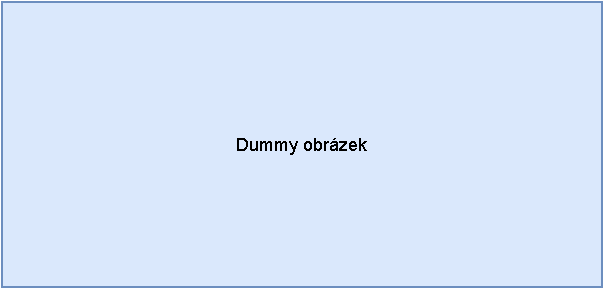
\includegraphics[width=3.0in, height=1.5in]{obrazky/dummy_pic.pdf}
	\caption{dummy obrázek - schéma transformer enkodéru}
	\label{transformer_encoder}
\end{figure}

Na obrázku \ref{transformer_encoder} můžeme vidět zjednodušenou strukturu jednotky enkodéru. V článku \cite{Transformers} tvoří enkodér 6 takových bloků propojených za sebe.\par
Před vstupem do prvního bloku jsou jednotlivé tokeny vstupního textu převedeny na vektory (word embeddings), ke kterým je přidáno poziční kódování\footnote{identifikuje pořadí tokenu ve vstupním textu.}.\par
Každý blok se pak skládá z \uv{multi-head attention} modulu a plně propojené dopředné vrstvy. Obě části jsou následovány normalizační vrstvou.\par
Nejzajímavější částí bloku enkodéru je multi-head attention modul, který je dále rozkreslen na obrázku \ref{multihead}. Modul je sofistikovanou implementací self-attention mechanismu popsaném dříve, který dokáže vyzdvihnout souvislost jednotlivých částí celého kontextu. 

\begin{figure}[hbt]
	\centering
	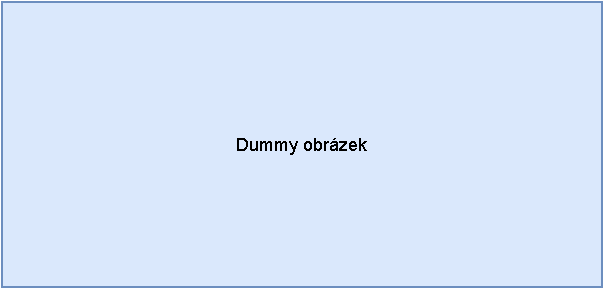
\includegraphics[width=0.45\linewidth, height=1.8in]{obrazky/dummy_pic.pdf}\hfill
	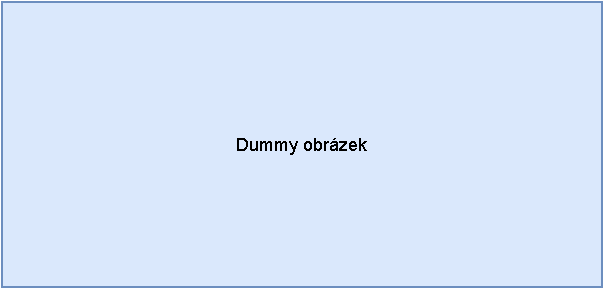
\includegraphics[width=0.45\linewidth, height=1.8in]{obrazky/dummy_pic.pdf}\hfill
	\caption{Obrázek multihead a scaled dot-product attention}
	\label{multihead}
\end{figure}

Mechanismus ne obrázku \ref{multihead} vlevo je popsaný rovnicí (\ref{attention_dot_product}) a je hlavním komponentem multi-head attention modulu znázorněném v \ref{multihead} vpravo.\par
Multi-head znamená, že do modulu vstupuje 8 (dle práce \cite{Transformers}) trojic V,K,Q. Každá matice trojice V,K,Q je transformována lieární vrstvou a na celou trojici je potom aplikován self dot-product attention (self-attention) mechanismus. Tento postup je aplikován na každou z osmi trojic paralelně, pokaždé však s jinými váhami lineární vrstvy.

%=========================================================================
\section{Předtrénované modely BERT a ALBERT}
\label{bert_albert}

V této sekci budou představeny modely založené na architektuře Transformer popsané v sekci \ref{transformers}. Informace v této sekci jsou převzaty z původních článků \cite{BERT} a \cite{ALBERT}.\par
Předtrénované modely stavějící na této architektuře určily nový standard pro přicházející state of the art metody. Kromě jejich vysoké úspěšnosti je obrovskou výhodou také znovupoužitelnost předtřénovaných modelů. Modely je možno jednoduše dotrénovat (provést tzv. \emph{fine-tuning} po načtení modelu s předtrénovanými parametry) pro celou řadu úkolů na poli NLP, jako je odpovídání na otázky, rozpoznání entit, klasifikace textu a další.

\subsection{BERT}
BERT (Bidirectional Encoder Representation from Transformers) je model pro reprezentaci přirozeného jazyka představený v roce 2018 prací \cite{BERT}. Jeho hlavním přínosem je aplikace obousměrného tréninku Transformer architektury. Ukazuje, že model trénovaný v obou směrech dokáže plně využít schopnost Transformerů zpracovávat vstupní text naráz, ne sekvenčně.\par\smallskip
Hlavním přínosem práce \cite{BERT} je způsob, kterým probíhá předtrénink na velkých textových korpusech. Trénink na úkolech, které nemusí přímo souviset s cílovým použitím dovolí modelu získat základní pochopení vlastností jazyka pro jeho správnou reprezentaci vytvořenou enkodérem. Pro předtrénink modelu BERT byly použity následující úkoly.

\begin{figure}[hbt]
	\centering
	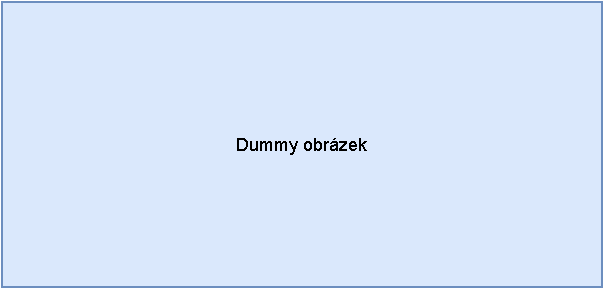
\includegraphics[width=0.45\linewidth, height=1.8in]{obrazky/dummy_pic.pdf}\hfill
	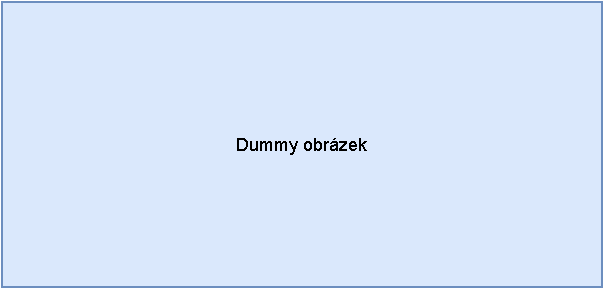
\includegraphics[width=0.45\linewidth, height=1.8in]{obrazky/dummy_pic.pdf}\hfill
	\caption{dummy obrázek - pre-training a fine-tuning berta}
	\label{bert}
\end{figure}

\medskip
\textbf{Maskované modelování jazyka} (ML modeling) 
je úloha velmi podobná již dříve zmíněné úloze predikce následujícího slova ve větě.Je ale použit přístup, kdy je určité procento slov v textu \emph{maskováno}, aby nebyl původní úkol kvůli obousměrné reprezentaci transformerů triviální.\par
Při tréninku je 15\,\% slov každé věty nahrazeno [MASK] tokenem, jehož původní význam je poté na základě okolního kontextu hádán.\par
Pro tento úkol je na enkodér BERTa napojena klasifikační vrstva, pomocí které je určena pravděpodobnost pro každého slovo ve slovníku, které má [MASK] token nahradit.\par
\smallskip
\textbf{Predikce následující věty} (NSP) je druhým typem úlohy pro předtrénink BERTa. Jeho snahou je naučit model porozumět vztahu nejen mezi jednotlivými slovy, ale taky mezi významem celých vět.\par
Trénovací dataset je rozdělen na dvojice vět A a B. Model má za úkol předpovědět, je-li věta B větou následující větu A v kontextu. V 50\,\% případů je věta B opravdu větou následující. Ve zbytku je to náhodně zvolená věta z korpusu.\par
Práce \cite{BERT} také uvádí, že navzdory jednoduchosti tohoto úkolu je jeho přínos pro pozdější aplikaci modelu pro odpovídání na otázky velký.\par

\paragraph{Formát vstupu}
modelu BERT je koncipován tak, aby mohl být použit pro větší spektrum aplikací, pro které je zamýšlen. Proto je umožněno na vstupu pomocí jediné sekvence tokenů reprezentovat jak jednu, tak i dvě vstupní sekvence, jako třeba otázku a odpověď.

\begin{figure}[hbt]
	\centering
	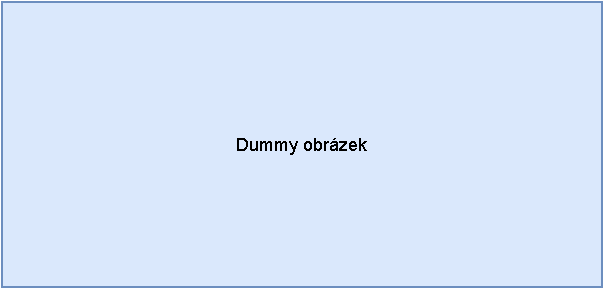
\includegraphics[width=5.0in, height=1.5in]{obrazky/dummy_pic.pdf}
	\caption{dummy obrázek - poziční, segmentové a token embeddings + special tokeny}
	\label{bert_input}
\end{figure}

Pro vektorovou reprezentaci jednotlivých tokenů jsou použity Wordpiece embeddings \cite{wordpiece} popsány v \ref{wordpiece_embb}. K těm je přidáno poziční kódování kvůli použití Transformer architektury a segmentační kódování, které identifikuje, které sekvenci vstupu jednotlivé tokeny náleží. Příklad je naznačen na obr. \ref{bert_input}.\par
Pro popis vstupu jsou navíc použity dva speciální tokeny [CLS] a [SEP]. [CLS] token je přidán vždy na začátek vstupu. Token [SEP] je přidán na konec každé sekvence. [CLS] token je využit také pro klasifikační úlohy (například předtrénink na NSP).

\subsection{ALBERT}
Informace v této sekci jsou převzaty ze článku \cite{ALBERT} \emph{A Lite BERT for self-supervised learning of language representations}.\par
Hlavním problémem modelu jako BERT je jeho velikost -- asi 110 milionů parametrů v jeho základní verzi. Zvětšováním modelu se většinou dá dosáhnout zlepšení, je to však problém kvůli omezené paměti grafických karet a množství času potřebného pro trénink.\par
\textbf{ALBERT} -- A Lite BERT, je model představený v roce 2019 článkem \cite{ALBERT}. Vychází z modelu BERT a dosahuje lepších výsledků na datových sadách pro porozumění textu, přestože má mnohem menší počet parametrů, než velká verze BERTa. V následujících odstavcích jsou shrnuty hlavní přínosy modelu ALBERT.

\paragraph{Faktorizace parametrů reprezentací} -- \emph{Factorized embedding parameterization}\\ 
\emph{Wordpiece embeddings} se učí reprezentovat tokeny nezávisle na kontextu, zatímco skryté vrstvy modelu se učí reprezentaci závislou na kontextu. Zvětšení velikosti skryté vrstvy způsobí u BERTa stejný nárůst velikosti reprezentace tokenů, jejichž význam není tak podstatný a model to zbytečně zatěžuje.
Díky odstranění provázanosti velikosti dimenze \emph{wordpiece embeddings} a dimenze skryté vrstvy modelu, je možno lépe zvětšovat velikost skrytých vrstev bez toho, aby to ovlivnilo velikost reprezentací ve slovníku.

\paragraph{Sdílení parametrů mezi vrstvami} -- \textit{Cross-layer parameter sharing}\\
Parametry napříč vrstvami jsou sdíleny, což zamezuje růstu počtu parametrů při zvětšování hloubky modelu a způsobuje jejich efektivnější využití. Ve výsledku má velká verze modelu ALBERT mnohonásobně méně parametrů, než velká verze modelu BERT.

\paragraph{Trénink návaznosti dvou vět} -- \textit{Inter-sentence coherence loss}\\
Trénink modelu BERT pomocí predikce následující věty (NSP) se částečně překrýval s úkolem predikce maskovaného tokenu, protože mohla být nesouvislost vět odhadnuta na základě nepříslušnosti slov stejnému tématu.\par
Pro trénink modelu ALBERT je pro tento úkol použita stejná dvojice vět A a B, u kterých se určuje, zda-li B navazuje na A. Při nenávaznosti však není věta B náhodně vybrána z jiného korpusu, ale je pouze prohozena s větou A. Model je tak lépe schopen naučit se logickou souvislost vět, místo odhadu tématu, ke kterému se věty vztahují bez toho, aby na sebe logicky navazovaly.
\bigskip\bigskip
\paragraph{ALBERT pro odpovídání na otázky}
Pro využití modelu ALBERT na konkrétní úkoly vyžadující porozumění textu je potřeba provést \emph{fine-tuning} modelu.\par
Pro odpovídání na otázky je na výstup modelu napojena lineání vrstva, která je natrénována na určení indexu začátku a konce odpovědi v rámci celé vstupní sekvence. Pro začátek a konec je poté vybrána validní\footnote{podmínky jako: start idx > end idx, odpověď se nenachází v první sekvenci (otázce)} dvojice indexů označující rozsah odpověď.\par
Pro \emph{fine-tuning} na daný úkol jsou optimalizovány parametry lineární klasifikační vrstvy i enkodéru ALBERT (vyžaduje delší trénink), nebo pouze lineární vrstvy.

%=========================================================================
%===============================================================================

\chapter{Řazení dokumentů dle relevance}
\label{document_indexing}
Tato kapitola popisuje metody pro indexaci a řazení dokumentů dle relevance, které jsou využity při vyhledávání relevantního dokumentu popsaného v části \ref{retriever_imp}. Nejprve bude vysvětlen význam indexu v kontextu řazení dokumentů a poté algoritmy, které ho využívají k vyhledávání. Nakonec budou diskutovány problémy velké báze dat jako je Wikipedie.\par
Informace v této kapitole jsou převzaty z prezentací Stanfordského kurzu \emph{Information Retrieval and Web Search}\footnote{Dostupné z: \url{https://web.stanford.edu/class/cs276/}} a knihy \emph{Introduction to Information Retrieval} \cite{information_retrieval}.

\section{Indexování dokumentů}
Pro vyhledávání dokumentů s použitím webových zdrojů jako Wikipedie jsou typické rozsáhlé texty které by bylo náročné procházet sekvenčně. Proto je důležité vytvořit strukturu, která je dále použita metodami pro řazení dokumentů a umožní optimalizované vyhledávání. Taková struktura se nazývá \textbf{index}.\par
Index poskytuje informace o výskytu jednotlivých termů v prohledávaných dokumentech a je vytvořen ještě před začátkem vyhledávání. Nejpoužívanější variantou je tzv. \emph{invertovaný index}.\par
Před vytvořením indexu je užitečné provést co nejlepší normalizaci prohledávaných dokumentů. Metody pro zpracování textu byly podrobně popsány v kapitole \ref{preprocessing} (převod na malá písmena, lemmatizace, odstranění stop slov).\par
\textbf{invertovaný index} je struktura obsahující všechny slova (termy) prohledávaného korpusu. Pro každý term je uložen seznam dokumentů (označených \emph{docID}), které daný výraz obsahují. Může obsahovat doplňující informace o počtu výskytů termu v dokumentu a jeho délce. Informace jsou poté využity při řazení dokumentů, tzv. \emph{ohodnoceném vyhledávání}.

\subsection{Úskalí velké báze dat jako Wikipedie}
Česká Wikipedie obsahuje velké množství článků (asi 3,5\,GB v nekomprimonavé podobě). Pro prohledávání celé Wikipedie je potřeba vytvořit a udržovat index, což je pro takový objem dat poměrně výpočetně a paměťově náročné. Je složité pomocí běžných nástrojů sestavit index pro celou Wikipedii.\par
Dalším problémem je různá délka dokumentů, nestrukturovanost některého textu a dynamicky se měnící prostředí, kdy jsou články na Wikipedii pravidelně aktualizovány.\par\enlargethispage{\baselineskip}
Způsoby prohledávání Wikipedie a vypořádání se se zmíněnými problémy jsou popsány v části \ref{design_and_implementation}, konkrétně \ref{design} a \ref{retriever_imp}.

%=========================================================================
\section{Algoritmy pro řazení dokumentů}
Při dotazování na vytvořený index nestačí výčet dokumentů, které termy přítomné v dotazu obsahují. Ohodnocené vyhledávání umožňuje získání pouze množiny seřazených \emph{n} nejvíce relevantních dokumentů.\par

\subsection{TF-IDF (Term frequency -- Inversed document frequency)}
\label{tf-idf}

\textbf{Četnost termu} (TF) je počet výskytů vyhledávaného termu v daném dokumentu. Vycházíme z předpokladu, že dokument s deseti výskyty termu bude pro dotaz více relevantní, než dokument obsahující vyhledávaný term pouze jednou. Neznamená to však, že bude dokument $10\times$ více relevantní -- růst relevance není přímo úměrný TF.\par
Jednotlivé termy nenesou stejnou informační hodnotu (např. stop slova \ref{stopwords}) a ojedinělé výrazy jsou často zásadní pro relevanci k dotazu (což souvisí i s neúměrným růstem relevance s růstem TF).\par

$$
    TF_{t,d} = log(1+tf_{t,d})
$$

\textbf{Četnost dokumentů} (DF) je počet dokumentů, které obsahují vyhledávaný term. Účel je v identifikaci termů vyskytujících se jenom ve zlomku dokumentů, které nejspíš ponesou zásadní informační hodnotu a adresovat tím neúměrnou závislost růst relevance dokumentu a četnosti termu. Obrácená četnost dokumentů (IDF) dělí celkový počet dokumentů \emph{N} četností dokumentů pro daný term. Hodnota IDF je tedy vyšší pro vzácnější termy.\par

$$
    IDF_{d} = log(\frac{N}{df_t})
$$

\textbf{TF-IDF} je statistická metoda, která použitím těchto dvou metrik hodnotí relevanci dokumentu.
Pro výpočet váhy TF-IDF pro daný term \emph{t} v dokumentu \emph{d} platí tedy:

$$
    \text{TF-IDF}_{t,d} = TF_{t,d} \cdot IDF_d
$$

Ohodnocení \emph{S} dokumentu \emph{d} pro dotaz \emph{q} je potom sumou jednotlivých ohodnocení termů \emph{t} dané otázky \emph{q}.

$$
    S(q,d) = \sum_{t\in{q \cap d}}^{}\text{TF-IDF}_{t,d}
$$

\subsection{BM25 (Best Match 25)}
\label{bm25}
(Okapi) BM25 představeno v \cite{bm25} je vylepšením klasické hodnotící funkce TF-IDF. Využívá poznatky statistiky a pravděpodobnosti pro řazení dokumentů dle jejich relevance s ohledem na vztah délky dokumntu a četnost výskytů termu v něm.\par
Delší dokumenty budou mít pravděpodobně větší $tf_{t,d}$. To je potřeba ve výsledném ohodnocení zohlednit, aby nebyly delší dokumenty nutně zvýhodněny.
Výsedný vzorec pro ohodnocení dokumentu \emph{d} pomocí BM25 vzhledem k otázce \emph{q} je:
$$
    S(q,d)^{BM25} = \sum_{t \in q} \left(IDF_d \cdot \frac{(k_1+1)\cdot tf_t}{k_1\cdot ((1-b)+b \cdot \frac{dl}{avdl}) + tf_t}\right)
$$
kde $tf$ a $idf$ jsou metriky vysvětlené v sekci \ref{tf-idf}, $dl$ je délka dokumentu $d$, $avdl$ je průměrná délka dokumentu v kolekci a $b,k_1$ jsou konstanty.
\begin{itemize}
    \item $k_1$ je konstanta ovlivňující dopad \emph{TF} na výsledné skóre dokumentu. Obvykle je volena v rozmezí $k_1\in(1,2 ;2)$. Pro nízké hodnoty $k_1$ roste význam dokumentu s rostoucí \emph{TF} poměrně rychle.
    \item $b$ ovlivňuje normalizaci délky dokumentu a obvykle je volena hodnota $b=0,75$. Hodnota $b=1$ znamená úplnou a $b=0$ žádnou normalizaci délky dokumentu.
\end{itemize}

Výhodu hodnotící funkce BM25 oproti obyčejnému TF-IDF lze demonstrovat na následujícím příkladu.\\ \medskip
Mějme vyhledávaný dotaz \uv{\emph{term frequency}} a dva dokumenty $d_1$ a $d_2$:\par

\begin{table}[H]
\centering
\begin{tabular}{|c|l|l|}
\hline
      & term & frequency \\ \hline
$d_1$ & 1024 & 1         \\ \hline
$d_2$ & 16   & 8         \\ \hline
\end{tabular}
\begin{tabular}{|c|l|l|}
\hline
      & \textbf{TF-IDF} & \textbf{BM25} \\ \hline
$d_1$ & \textbf{87} & 31         \\ \hline
$d_2$ & 75 & \textbf{43}         \\ \hline
\end{tabular}
\caption{Výskyt termů \uv{term} a \uv{frequency} v dokumentech $d_1$ a $d_2$ a ohodnocení jednotlivých dokumentů podle funkcí TF-IDF a BM25 ($k_1 = 2$)}
\label{tab:tf}
\end{table}

Tabulka \ref{tab:tf} ukazuje, jak BM25 lépe zohlednilo počet výskytů termů a skutečně ohodnotilo lépe relevantnější dokument.\par \medskip
Pro BM25 existují také modifikace, jako BM25+, BM25L a další, které byly porovnány v \cite{bm25_improvements}.\par
\begin{itemize}
    \item BM25L \cite{bm25_too_long} adresuje znevýhodnění příliš dlouhých dokumentů klasickou BM25 funkcí.
    \item BM25+ \cite{bm25_plus} adresuje stejný problém jako BM25L, ale implementuje vylepšení odlišně
\end{itemize}
Závěr článku \cite{bm25_improvements} ale ukazuje, že neexistuje modifikace, která by systematicky zlepšila dosažené výsledky vyhledávání.\par


%=========================================================================
%===============================================================================

\chapter{Dostupné datové sady a výběr}
\label{available_datasets}
Tato kapitola se zabývá popisem a výběrem datových sad (datasetů) pro realizaci a evaluaci systému.\par
Datová sada je v oblasti strojového učení velká anotovaná (člověkem popsaná) kolekce dat pro trénink a vyhodnocování neuronových sítí. Obvykle obsahuje pro každý příklad vstupní data a jejich popis (anotaci).\\
Datové sady je možno rozdělit podle toho, v jaké fázi vývoje s nimi pracujeme.
\begin{itemize}
    \item \textbf{Trénovací} Používá se pro naučení neuronové sité. Při zpracovávání trénovací datové sady se model učí a upravuje své parametry. Na konci tréninku by měl model konvergovat ke 100\,\% úspěšnosti na trénovací datové sadě.
    \item \textbf{Validační} Slouží pro průběžné vyhodnocení existujícího modelu v průběhu vývoje. Model se z validačních dat neučí. Může být využit například k úpravě hyperparametrů nebo zastavení tréninku modelu, když se jeho úspěšnost na validační datové sadě přestane zlepšovat. Vytvořen může být vybraným zlomkem trénovacího datasetu nepoužitým pro trénink.
    \item \textbf{Testovací} Obsahuje příklady z reálného světa, na kterých je model/systém vyhodnocen po dokončení jeho vývoje. Testovací dataset je často shodný s validačním.
\end{itemize}
Pro trénink neuronových sítí pro odpovídání na otázky by měla datová sada obsahovat hlavně:
\begin{itemize}
    \item otázku
    \item kontext (dokument obsahující odpověď)
    \item odpověď
    \item případně doplňující informace (jako začátek odpovědi, délku odpovědi \dots)
\end{itemize}
Vytvoření takové datové sady je složitý úkol vyžadující velké množství lidských zdrojů. Je potřeba nasbírat dostatečné množství dokumentů, pro které někdo musí vymyslet otázky a vyznačit v dokumentech příslušné odpovědi. Tvorba datových sad obvykle probíhá pomocí \emph{crowdsourcingu}\footnote{\emph{Crowdsourcing je nové slovo označující proces získání potřebné služby, nápadů, příspěvků, pomoci při řešení problémů od velké skupiny lidí.} (\url{https://wikisofia.cz/wiki/Crowdsourcing})}.

%=========================================================================
\section{Datové sady pro angličtinu}
Pro angličtinu existuje celá řada datových sad zaměřených na odpovídání na otázky. Nejznámější z nich je však SQuAD (\emph{Stanford Question Answering Dataset}) \cite{squad}. Dataset obsahuje asi 100 000 anotovaných dvojic otázka--odpověď z více jak 500 různých článků z anglické Wikipedie. Existuje také rozšířená verze SQuAD datasetu. SQuAD2.0 \cite{squad_v2} obsahuje navíc 50 000 otázek, na které v kontextu neexistuje odpověď. Model tedy musí umět určit, když dokument odpověď neobsahuje.

%=========================================================================
\section{Datové sady pro češtinu}
Čeština nabízí poměrně omezené zdroje oproti anglickým datovým sadám.\par 
Nejznámější je datová sada SQADv3 (Simple Question Answering Database) \cite{sqad}. Obsahuje přes 13 000 příkladů otázek s odpovědí v přiloženém kontextu pocházejícím z české Wikipedie. Datová sada otázky směřované na časový údaj, entitu, lokaci, osobu \dots \,včetně 16\,\% ano/ne otázek.\par
Existuje také česká verze anglického datasetu SQuAD prezentovaná v práci \cite{czech_squad}. Datová sada je strojovým překladem původního datasetu SQuAD 1.1 a SQuAD2.0. Oproti anglické verzi však obsahuje asi 70 000 otázek pro první (1.1) a 110 000 otázek pro druhou (2.0) verzi datové sady SQUAD. Ztráta části rozsahu datové sady je způsobena problémy s vyznačením odpovědi ve strojově přeložené verzi dokumentu.

%=========================================================================
\section{Výběr trénovacích a testovacích dat}
\label{dataset_choice}
Pro systém je potřeba vybrat data pro natrénování modelů pro vyznačení odpovědi v získaném textu a pro validaci výsledného systému.\par
Pro trénink anglického modelu byl vybrán anglický SQuAD 1.1 (obsahující i validační část datasetu). Po zvážení bylo rozhodnuto použít první verzi datasetu, protože budou testovací data obsahovat pouze otázky, pro které existuje na otevřené doméně odpověď.\par
Pro trénink českého modelu byl vybrán český překlad anglického datasetu SQuAD 1.1 \cite{czech_squad} kvůli jeho velikosti a porovnatelnosti s anglickou verzí datové sady.\par
\medskip
Jako testovací datová sada byl zvolen český dataset SQADv3, ze kterého bylo odstraněno 16\,\% otázek očekávajících ano/ne odpovědi. Datová sada nejlépe odpovídá reálnému scénáři užití systému, protože obsahuje otázky a odpovědi z článků z české Wikipedie (narozdíl od trénovacích datasetů).


%=========================================================================
%===============================================================================

\chapter{Návrh systému a implementace jednotlivých komponent}
\label{design_and_implementation}
V této kapitole je rozebrán návrh systému a implementace jeho částí. Nejprve je popsán zvolený přístup k řešení problému a rozdělení problému na části reprezentující blokové schéma celého systému. Následuje popis nástrojů a knihoven použitých pro implementaci jednotlivých komponent. Nejdůležitější částí jsou sekce o implementaci dvou hlavních nezávislých částí \ref{reader} a \ref{retriever_imp}. Nakonec je shrnut výsledný tok programu pro odpovídání na otázky nad českou Wikipedií.

\begin{figure}[hbt]
	\centering
	\scalebox{1.2}{
	    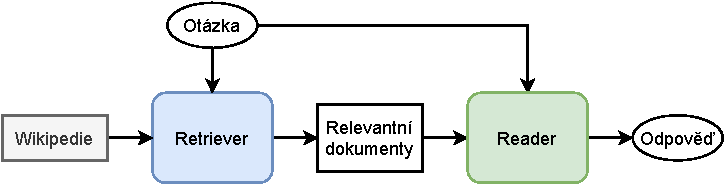
\includegraphics{obrazky/reader-retriever-scheme.pdf}
	}
	\caption{Generické schéma (prezentované například v \cite{drQA}) open-domain QA systému}
	\label{qa_scheme}
\end{figure}

%=========================================================================
\section{Zvolený přístup k problému}
Odpovídání na otázky na otevřené doméně (open-domain QA) má obvykle dvě hlavní (na sobě téměř nezávislé) části, jak je naznačeno na obrázku \ref{qa_scheme}. První částí je \emph{Retriever}, který má za úkol získat z internetu (pro nás z Wikipedie) relevantní dokumenty, které by mohly obsahovat odpověď a druhou je \emph{Reader}, který provede extrakci odpovědi ze získaného kontextu \cite{drQA}.\par
\noindent\emph{Retriever} části systému je věnována pozornost v sekci \ref{retriever_imp}.\par
Pro návrh systému bylo však největší dilema v realizaci \emph{Reader} části systému pro kvalitní extrakci odpovědi v češtině. Chtěl jsem využít některého z populárních předtrénovaných modelů (\ref{bert_albert}) založených na Transformers \cite{Transformers} architektuře (\ref{transformers}). Proto jsem se rozhodl vyzkoušet přístup, kdy je nativně anglickému ALBERT modelu, který dosahuje špičkových výsledků\footnote{\url{https://rajpurkar.github.io/SQuAD-explorer/}}, strojově přeložen vstupní dokument i otázka z češtiny do angličtiny.\par
Pro porovnání jsem zvolil vícejazyčný model BERTa (m-BERT\footnote{\url{https://github.com/google-research/bert/blob/master/multilingual.md}}), který podporuje 104 světových jazyků s nejrozsáhlejší Wikipedií, trénovaný na českém překladu datové sady SQuAD 1.1 \cite{czech_squad} \cite{squad}.\par

%=========================================================================
\section{Návrh jednotlivých částí systému}
\label{design}
V této sekci bude popsán návrh systému, tedy hlavně \emph{Retrieveru}, \emph{Readeru} a části pro zpracování datové sady SQAD v3.0 \cite{sqad} pro závěrečné vyhodnocení.

\subsection{Návrh Retrieveru}
Získání \emph{n} relevantních dokumentů kandidujících pro zodpovězení otázky vyžaduje několik na sebe navazujících kroků (obrázek \ref{retriever-simple-scheme}). V návrhu a implementaci jsou použity metody předzpracování textu a řazení dokumentů popsané v kapitolách \ref{text_processing} a \ref{document_indexing}.\par
Retriever dostává na vstupu otázku, která je také hlavním vstupem do celého systému. Dříve, než se na základě otázky začnou přímo prohledávat odstavce české Wikipedii, bude dobré z otázky získat co nejvíce informací, které by mohly vést ke \emph{spraveným článkům}. Až po jejich získání jsou jednotlivé články rozděleny na odstavce a ty prohledávány.\par
\noindent K získání článku jsou použity tři metody:
\begin{itemize}
    \item \textbf{základní Wiki Search} nezpracované otázky, který někdy přináší uspokojivé výsledky, ale většinou je nedostačující,
    \item \textbf{získání relevantního titulku článku} (pomocí BM25 \ref{bm25}) z \emph{dumpu} titulků\footnote{\url{https://cs.wikipedia.org/wiki/Wikipedie:St\%C3\%A1hnut\%C3\%AD_datab\%C3\%A1ze}} české Wikipedie po lemmatizaci otázky a odstranění stop slov,
    \item \textbf{rozpoznání (pojmenované) entity}, která by se mohla vyskytovat v titulku článku a usnadnit tím \emph{Wiki Search}.
\end{itemize}
Tímto tedy získáme seznam článků z Wikipedie, který je následně upraven tak, aby se v něm každý získaný článek vyskytoval pouze jednou.\par
Jednotlivé články je následně třeba rozdělit na odstavce, normalizovat jejich délku, lemmatizovat je, odstranit stop slova a indexovat je. Odstavce jsou poté seřazeny algoritmem BM25 a z nich vybrány první tři nejvhodnější. Pro vyhledávání mezi odstavci je použita lemmatizovaná otázka s odstraněnými stop slovy. Tři nejvhodnější odstavce jsou získány v jejich původní, nezpracované podobě a případně (při použití nativně anglického \emph{readeru}) jsou včetně otázky přeloženy do angličtiny.

\begin{figure}[hbt]
	\centering
	\scalebox{0.9}{
	    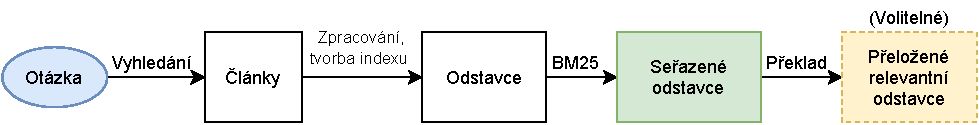
\includegraphics{obrazky/retriever-simple-scheme.pdf}
	}
	\caption{Zjednodušené schéma \emph{retriever} části systému}
	\label{retriever-simple-scheme}
\end{figure}

Následuje podrobný návrh struktury \emph{retrieveru} znázorňující podrobně jednotlivé komponenty na obrázku \ref{retriever-podrobne}.

\begin{figure}[hbt]
    \centering
	\scalebox{0.9}{
	    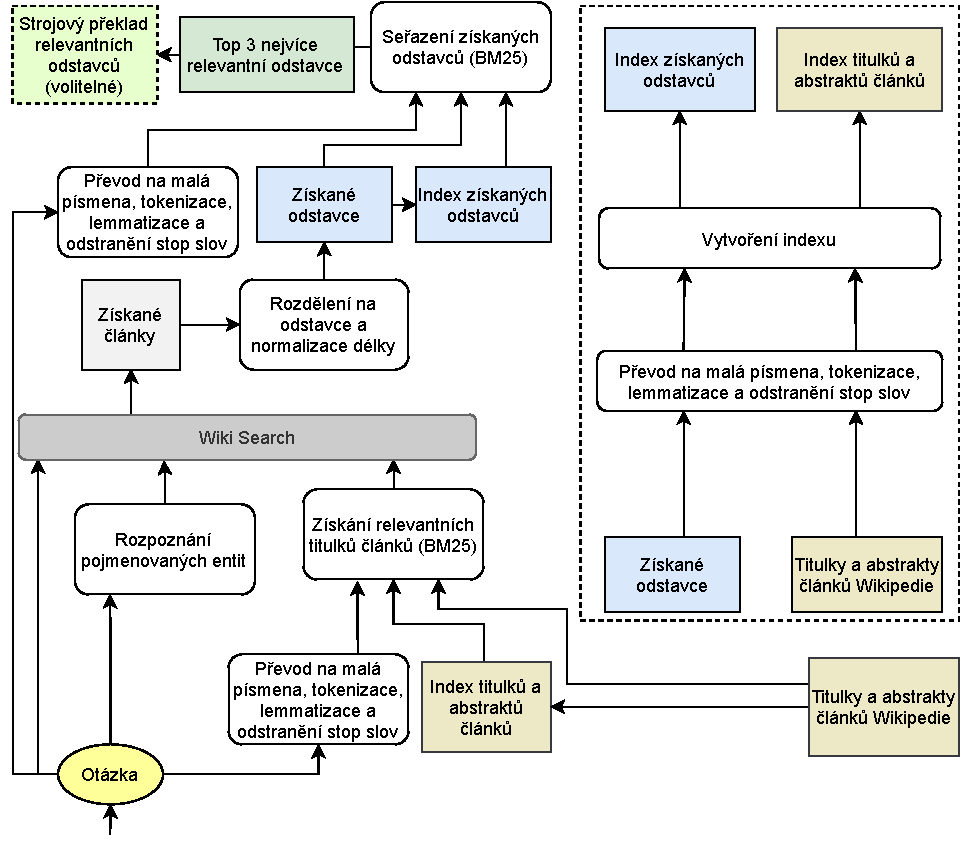
\includegraphics{obrazky/retriever_podrobne.pdf}
	}
	\caption{Podrobné schéma \emph{retriever} části systému}
	\label{retriever-podrobne}
\end{figure}

\subsection{Návrh Readeru}
Část systému pro extrakci odpovědi ze získaného dokumentu byla navržena ve dvou variantách.
\begin{itemize}
    \item \textbf{Anglický ALBERT} s lineární klasifikační vrstvou pro určení začátku a konce odpovědi, pro který jsou vstupní dokumenty a otázka strojově přeloženy do angličtiny. Výsledná odpověď je přeložena opět zpět do češtiny.
    \item \textbf{Vícejazyčný BERT (m-BERT)} opět s lineární klasifikační vrstvou pro určení začátku a konce odpovědi, který dokáže odpovídat přímo na českých dokumentech.
\end{itemize}
Pro obě varianty je však postup (až na překlad pro anglický ALBERT, který je však součástí \emph{retrieveru}) shodný.\par
Model dostane k přečtení tři nejvíce relevantní odstavce získané \emph{retrieverem}. Pro každý odstavec je provedena extrakce odpovědi, kdy je vybrána vždy právě jedna validní odpověď s největším \uv{skóre}(nenormalizovaná logaritmická pravděpodobnost) pro daný dokument. Ze získaných odpovědí je vybrána ta, kterou si je model nejvíce jistý (ta s největším skóre) a případně (při použití ALBERT-en modelu) přeložena zpátky do češtiny.\par
\noindent Ostatní odpovědi jsou také uloženy pro získání statistických dat při vyhodnocení. \emph{Reader} tak vybere kromě odpovědi také finální dokument, ze kterého je odpověď získána, který může být použit pro získání některých dalších informací/kontextu uživatelem.\par
Schéma \emph{readeru} pro extrakci finální odpovědi je naznačeno na obrázku \ref{reader_schema}. Modely použité k implementaci a naznačeny v návrhu byly blíže popsány v kapitole \ref{language_comprehension}, konkrétně v sekci \ref{bert_albert}.

\begin{figure}[hbt]
	\centering
	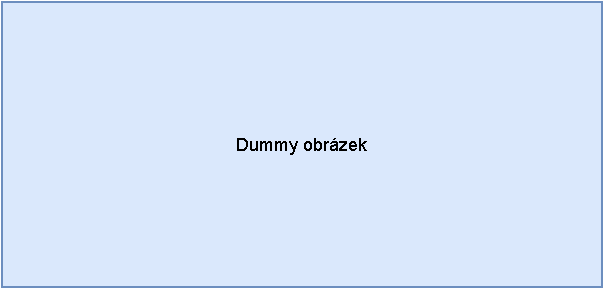
\includegraphics[width=5.0in, height=3.5in]{obrazky/dummy_pic.pdf}
	\caption{dummy obrázek - schéma reader části systému}
	\label{reader_schema}
\end{figure}


\subsection{Návrh vyhodnocení}

\subsection{Popis výsledného systému}
%=========================================================================
\section{Použité nástroje a technologie pro implementaci}
\label{pouzite_nastroje}


%=========================================================================
\section{Implementace a trénink readeru}
\label{reader}


%=========================================================================
\section{Implementace retrieveru}
\label{retriever_imp}


%=========================================================================



%=========================================================================
%===============================================================================

\chapter{Vyhodnocení systému a rozbor chyb}
\label{system_evaluation}



%=========================================================================
\section{Vysvětlení základních metrik}


%=========================================================================
\section{Postup při vyhodnocování výsledného systému}


%=========================================================================
\section{Porovnání výsledků se současným stavem poznání}


%=========================================================================
\section{Rozbor chyb a možnosti dalšího vývoje}



%=========================================================================
%===============================================================================

\chapter{Závěr}
\label{conclusion}


%=========================================================================
%===============================================================================
